\documentclass[11pt]{article}

% ===================== PAQUETES =====================
\usepackage[utf8]{inputenc}
\usepackage[spanish,es-noquoting]{babel}
\shorthandoff{.}
\usepackage[T1]{fontenc}
\usepackage[margin=2.5cm]{geometry}
\usepackage{titlesec}
\usepackage{booktabs}
\usepackage{array}
\usepackage{xcolor}
\usepackage{hyperref}
\usepackage{fancyhdr}
\usepackage{enumitem}
\usepackage{parskip}
\usepackage{listings}
\usepackage{graphicx}
\usepackage{caption}

% ===================== COLORES =====================
\definecolor{primario}{RGB}{27,79,114}
\definecolor{secundario}{RGB}{46,139,87}
\definecolor{fondocodigo}{RGB}{245,245,245}

% ===================== ESTILO DE CÓDIGO =====================
\lstdefinestyle{python}{
    language=Python,
    backgroundcolor=\color{fondocodigo},
    basicstyle=\ttfamily\footnotesize,
    keywordstyle=\color{primario}\bfseries,
    commentstyle=\color{secundario}\itshape,
    stringstyle=\color{orange!70!black},
    numbers=left,
    numberstyle=\tiny\color{gray},
    breaklines=true,
    frame=single,
    rulecolor=\color{gray!40},
    showstringspaces=false,
    tabsize=4,
    literate=
        {á}{{\'a}}1 {é}{{\'e}}1 {í}{{\'i}}1 {ó}{{\'o}}1 {ú}{{\'u}}1
        {Á}{{\'A}}1 {É}{{\'E}}1 {Í}{{\'I}}1 {Ó}{{\'O}}1 {Ú}{{\'U}}1
        {ñ}{{\~n}}1 {Ñ}{{\~N}}1 {ü}{{\"u}}1
}
\lstset{style=python}

% ===================== ESTILO DE SECCIONES =====================
\titleformat{\section}
  {\Large\bfseries\color{black}}{\thesection}{1em}{}
\titleformat{\subsection}
  {\large\bfseries\color{black}}{\thesubsection}{1em}{}

% ===================== ENCABEZADO/PIE =====================
\pagestyle{fancy}
\fancyhf{}
\renewcommand{\headrulewidth}{0.4pt}
\fancyhead[L]{\small Energías Renovables y Emisiones de CO\textsubscript{2} en Colombia}
\fancyhead[R]{\small Informe Final}
\fancyfoot[C]{\small\thepage}

% ===================== ENLACES =====================
\hypersetup{
    colorlinks=true,
    linkcolor=primario,
    urlcolor=primario,
    citecolor=primario
}

\captionsetup{labelfont=bf, font=small}

\begin{document}

% ===================== PORTADA =====================
\begin{titlepage}
    \centering
    \vspace*{2cm}
    {\Huge\bfseries\color{black} Análisis de la Relación entre las Energías Renovables y las Emisiones de CO\textsubscript{2} en Colombia (1990--2021)\par}
    \vspace{1.5cm}
    {\Large Informe Final -- Proyecto de Ciencia de Datos\par}
    \vspace{2cm}
    {\large\bfseries Integrantes\par}
    \vspace{0.3cm}
    {\large
    Juan Castillo \\
    Maira Martínez \\
    Jorge Bernal \\
    Samuel Solano \par}
    \vspace{2cm}
    {\large Docente: Camila Silva Gómez\par}
    \vspace{0.3cm}
    {\large Universidad EAN\par}
    \vspace{0.3cm}
    {\large Bogotá, Colombia \par}
    \vfill
    {\large \today\par}
\end{titlepage}

\tableofcontents
\newpage

% ===================== 1. PLANTEAMIENTO DEL PROBLEMA =====================
\section{Planteamiento del Problema y Objetivo del Proyecto}

Colombia cuenta con una de las matrices eléctricas más limpias de América Latina, con una participación de energías renovables (principalmente hidroeléctrica) que se ha mantenido por encima del 60\% durante todo el periodo 1990--2021. Sin embargo, en ese mismo periodo las emisiones totales de CO\textsubscript{2} del país casi se duplicaron, pasando de 56.9 a 103.7 millones de toneladas. Esta aparente contradicción —una matriz eléctrica mayoritariamente renovable conviviendo con un crecimiento sostenido de las emisiones— motiva la pregunta central de este proyecto.

\subsection*{Pregunta de investigación}
\textit{¿Qué relación existe entre el crecimiento de las energías renovables y las emisiones de CO\textsubscript{2} en Colombia entre 1990 y 2021?}

\subsection*{Objetivo general}
Determinar el tipo y la magnitud de la relación entre la participación de energías renovables en la matriz eléctrica y las emisiones de CO\textsubscript{2} per cápita en Colombia, mediante análisis estadístico y modelos de aprendizaje automático aplicados a series de tiempo del periodo 1990--2021.

\subsection*{Objetivos específicos}
\begin{itemize}[leftmargin=1.2cm]
    \item Caracterizar la evolución histórica de las emisiones de CO\textsubscript{2}, el consumo de energía y la participación renovable en Colombia.
    \item Cuantificar la correlación entre la participación de renovables, el consumo de energía per cápita y las emisiones de CO\textsubscript{2} per cápita.
    \item Construir y comparar modelos predictivos que estimen las emisiones de CO\textsubscript{2} per cápita a partir de variables energéticas.
    \item Identificar cuál de las dos variables predictoras (renovables o consumo energético) tiene mayor peso en la explicación de las emisiones.
\end{itemize}

% ===================== 2. BÚSQUEDA Y OBTENCIÓN DE DATOS =====================
\section{Búsqueda y Obtención de los Datos}

\subsection*{Fuente de los datos}
La información utilizada proviene de dos conjuntos de datos públicos publicados por \textbf{Our World in Data (OWID)}, alojados en su repositorio oficial de GitHub:

\begin{itemize}[leftmargin=1.2cm]
    \item \textbf{CO2 and Greenhouse Gas Emissions Dataset}: \url{https://github.com/owid/co2-data}
    \item \textbf{Energy Dataset}: \url{https://github.com/owid/energy-data}
\end{itemize}

\subsection*{Justificación de la fuente}
Se seleccionaron estas fuentes porque: (1) son bases de datos abiertas y de acceso público, sin restricciones de uso académico; (2) se actualizan periódicamente y están respaldadas por instituciones como el Global Carbon Project y la Energy Institute; (3) son ampliamente utilizadas en investigación académica sobre energía y cambio climático, lo que otorga trazabilidad y confiabilidad; y (4) permiten acceso directo por URL, lo que garantiza la reproducibilidad total del proyecto sin depender de archivos locales.

\subsection*{Método de obtención}
Los datos se cargaron directamente en Python mediante \texttt{pandas.read\_csv()} apuntando a la URL cruda (\textit{raw}) de cada archivo en GitHub, sin necesidad de descarga manual. De ambos conjuntos se extrajeron únicamente los registros correspondientes a \textbf{Colombia} en el rango de años \textbf{1990--2021}.

% ===================== 3. COMPRENSIÓN DEL DATASET =====================
\section{Comprensión del Conjunto de Datos y Descripción de las Variables}

Los datasets originales de OWID contienen decenas de variables para todos los países del mundo. Para este proyecto se filtraron y seleccionaron únicamente las variables relevantes para la pregunta de investigación. Tras el proceso de limpieza, la tabla analítica final (\texttt{df\_clean}) quedó conformada por:

\begin{center}
\begin{tabular}{@{}p{3.3cm}p{9.5cm}@{}}
\toprule
\textbf{Variable} & \textbf{Descripción} \\
\midrule
\texttt{Year} & Año de observación (1990--2021). \\
\texttt{CO2\_Mt} & Emisiones totales de CO\textsubscript{2} de Colombia, en millones de toneladas (Mt). \\
\texttt{CO2\_per\_capita} & Emisiones de CO\textsubscript{2} por habitante, en toneladas por persona. \\
\texttt{Renewables\_pct} & Porcentaje de electricidad generada a partir de fuentes renovables. \\
\texttt{Energy\_per\_capita} & Consumo de energía primaria por habitante. \\
\texttt{population} & Población total de Colombia para el año correspondiente. \\
\bottomrule
\end{tabular}
\end{center}

La unidad de análisis es el año-país (Colombia), con 32 observaciones (1990 a 2021), sin valores nulos ni duplicados en el rango seleccionado.

% ===================== 4. LIMPIEZA Y PREPROCESAMIENTO =====================
\section{Proceso de Limpieza y Preparación de los Datos}

El tratamiento de los datos se realizó en Python (\texttt{pandas}) siguiendo los pasos que se describen a continuación:

\begin{enumerate}[leftmargin=1.2cm]
    \item \textbf{Carga de datos:} lectura directa de los archivos \texttt{owid-co2-data.csv} y \texttt{owid-energy-data.csv} desde el repositorio oficial de OWID en GitHub.
    \item \textbf{Filtrado:} de cada dataset se conservaron únicamente los registros donde \texttt{country == "Colombia"} y el año estuviera entre 1990 y 2021.
    \item \textbf{Selección y renombrado de columnas:} se conservaron las variables relevantes de cada fuente (\texttt{co2}, \texttt{population} del dataset de emisiones; \texttt{renewables\_share\_elec}, \texttt{primary\_energy\_consumption} del dataset de energía), renombrándolas a nombres más descriptivos.
    \item \textbf{Unión de tablas:} los dos subconjuntos se combinaron mediante un \textit{merge} por la columna \texttt{year}, generando una única tabla (\texttt{df\_colombia}) con todas las variables alineadas por año.
    \item \textbf{Cálculo de variables per cápita:} a partir de las variables absolutas y la población, se calcularon \texttt{CO2\_per\_capita} y \texttt{Energy\_per\_capita}, para permitir comparaciones normalizadas por habitante.
    \item \textbf{Estandarización de nombres:} la columna \texttt{year} se renombró a \texttt{Year} para mantener consistencia en el resto del análisis.
    \item \textbf{Consolidación final:} se construyó la tabla analítica \texttt{df\_clean}, con las seis variables finales listas para el análisis exploratorio, estadístico y de modelado.
    \item \textbf{Exportación:} la base limpia se exportó a un archivo Excel (\texttt{datos\_limpios\_colombia\_1990\_2021.xlsx}) para su respaldo y consulta.
\end{enumerate}

\subsection*{Fragmento de código: filtrado, unión y cálculo per cápita}

\begin{lstlisting}
# Filtrado por pais y periodo (1990-2021)
col_co2 = df_co2_raw[(df_co2_raw['country'] == 'Colombia') &
                      (df_co2_raw['year'].between(1990, 2021))].copy()

# Seleccion y renombrado de columnas relevantes
col_co2 = col_co2[['year', 'co2', 'population']].rename(
    columns={'co2': 'CO2_Mt'})
col_energy = col_energy[['year', 'renewables_share_elec',
                          'primary_energy_consumption']].rename(
    columns={'renewables_share_elec': 'Renewables_pct',
             'primary_energy_consumption': 'Energy_TWh'})

# Union de las dos fuentes de datos por año
df_colombia = pd.merge(col_co2, col_energy, on='year')

# Calculo de variables per capita
df_colombia['CO2_per_capita'] = (df_colombia['CO2_Mt'] * 1e6) / df_colombia['population']
df_colombia['Energy_per_capita'] = (df_colombia['Energy_TWh'] * 1e9) / df_colombia['population']
\end{lstlisting}

% ===================== 5. EDA =====================
\section{Análisis Exploratorio de Datos (EDA)}

\subsection*{Evolución de las emisiones de CO\texorpdfstring{\textsubscript{2}}{2}}
Las emisiones totales de CO\textsubscript{2} muestran una tendencia creciente sostenida, con una caída puntual a finales de los años 90 (crisis económica de 1999) y una aceleración marcada a partir de 2005.

\begin{figure}[h!]
    \centering
    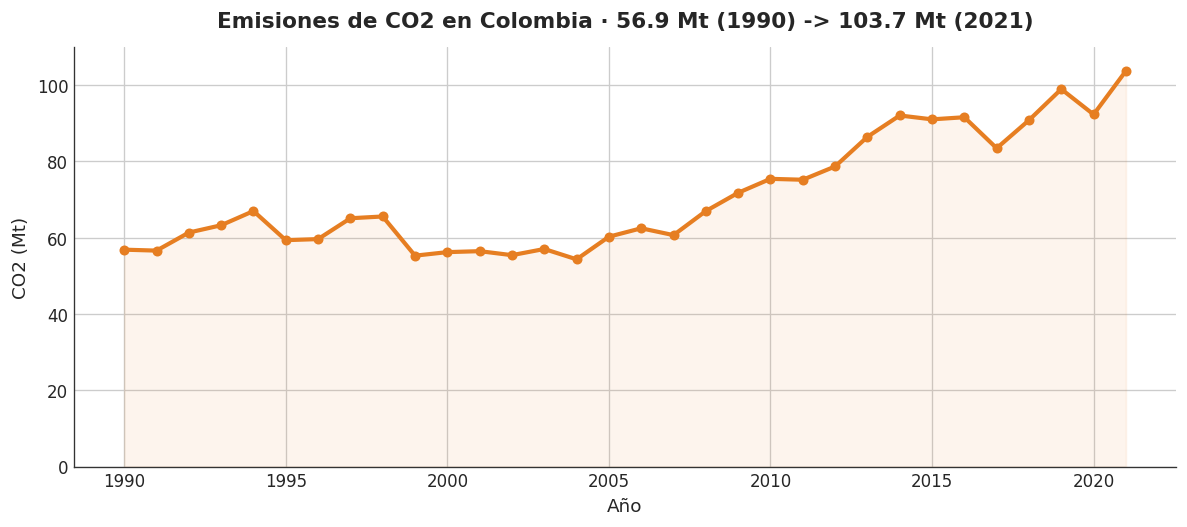
\includegraphics[width=0.85\textwidth]{figuras/co2_tendencia.png}
    \caption{Emisiones de CO\textsubscript{2} en Colombia, 1990--2021.}
\end{figure}

\subsection*{Evolución de la participación renovable}
La electricidad renovable se mantiene siempre por encima del 60\%, con oscilaciones marcadas en años como 1992 y 2015--2016, coincidentes con periodos de sequía asociados al fenómeno de El Niño, que reduce la generación hidroeléctrica y obliga a un mayor uso de térmicas.

\begin{figure}[h!]
    \centering
    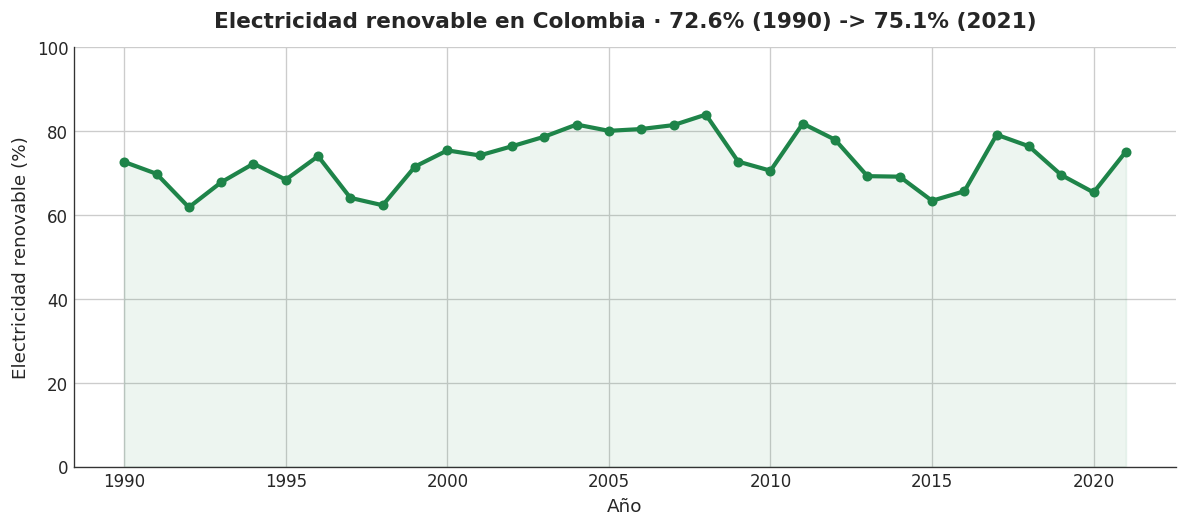
\includegraphics[width=0.85\textwidth]{figuras/renovables_tendencia.png}
    \caption{Participación de electricidad renovable en Colombia, 1990--2021.}
\end{figure}

\newpage
\subsection*{Estadística descriptiva}

\begin{center}
\begin{tabular}{@{}lccccccc@{}}
\toprule
\textbf{Variable} & \textbf{Media} & \textbf{Mediana} & \textbf{Moda*} & \textbf{Desv. Est.} & \textbf{Asimetría} & \textbf{Mínimo} & \textbf{Máximo} \\
\midrule
CO2\_Mt              & 70.98   & 65.33   & 57.0   & 15.10   & 0.72  & 54.32  & 103.73 \\
CO2\_per\_capita      & 1.68    & 1.72    & 2.0    & 0.21    & -0.17 & 1.31   & 2.03   \\
Renewables\_pct       & 72.86   & 72.65   & 69.0   & 6.24    & -0.07 & 61.78  & 83.89  \\
Energy\_per\_capita   & 9372.31 & 9144.85 & 9041.0 & 1276.98 & 0.46  & 7783.00& 11652.96\\
\bottomrule
\end{tabular}
\end{center}
\textit{*Moda calculada sobre valores redondeados.}

Las emisiones de CO\textsubscript{2} totales presentan asimetría positiva moderada (0.72), reflejando el crecimiento acelerado de los últimos años del periodo. La participación renovable, en cambio, es la variable más estable (coeficiente de variación de apenas 8.6\%), lo que sugiere que su rol como \textit{driver} directo del crecimiento de emisiones es limitado: no es la variable que más cambia en el tiempo.

% ===================== 6. ANÁLISIS ESTADÍSTICO =====================
\section{Análisis Estadístico}

Se calculó la matriz de correlación de Pearson entre las cuatro variables numéricas principales:

\begin{figure}[h!]
    \centering
    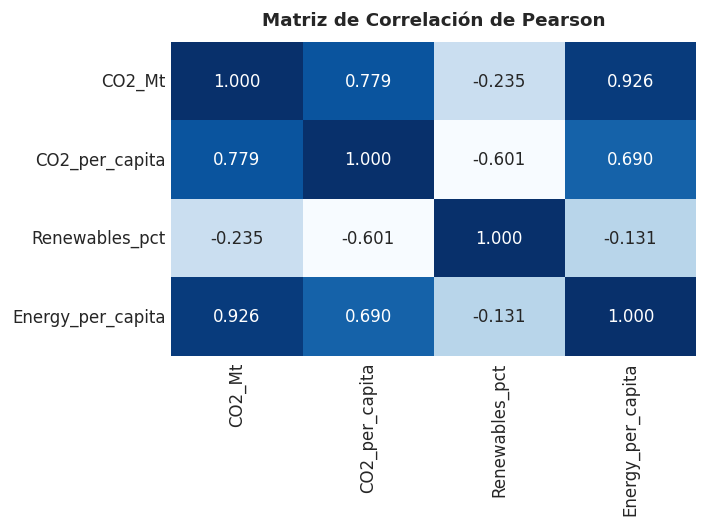
\includegraphics[width=0.6\textwidth]{figuras/matriz_correlacion.png}
    \caption{Matriz de correlación de Pearson.}
\end{figure}

Los resultados más relevantes son:

\begin{itemize}[leftmargin=1.2cm]
    \item \textbf{Energy\_per\_capita vs. CO2\_Mt}: \textit{r} = 0.926 (correlación positiva muy fuerte).
    \item \textbf{Energy\_per\_capita vs. CO2\_per\_capita}: \textit{r} = 0.690 (correlación positiva moderada-alta).
    \item \textbf{Renewables\_pct vs. CO2\_per\_capita}: \textit{r} = -0.601 (correlación negativa moderada).
    \item \textbf{Renewables\_pct vs. CO2\_Mt}: \textit{r} = -0.235 (correlación negativa débil).
\end{itemize}

\begin{figure}[h!]
    \centering
    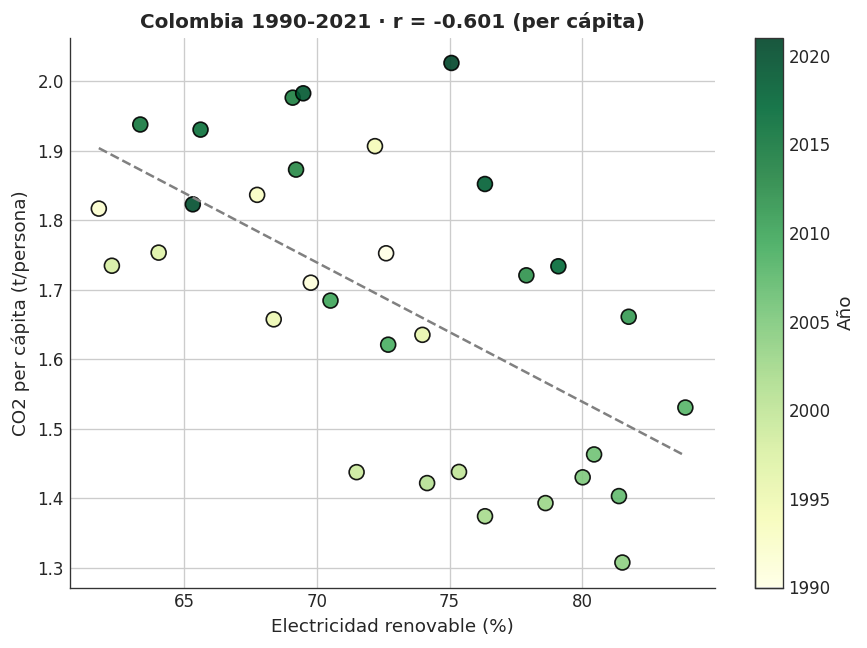
\includegraphics[width=0.48\textwidth]{figuras/scatter_renovables_co2.png}
    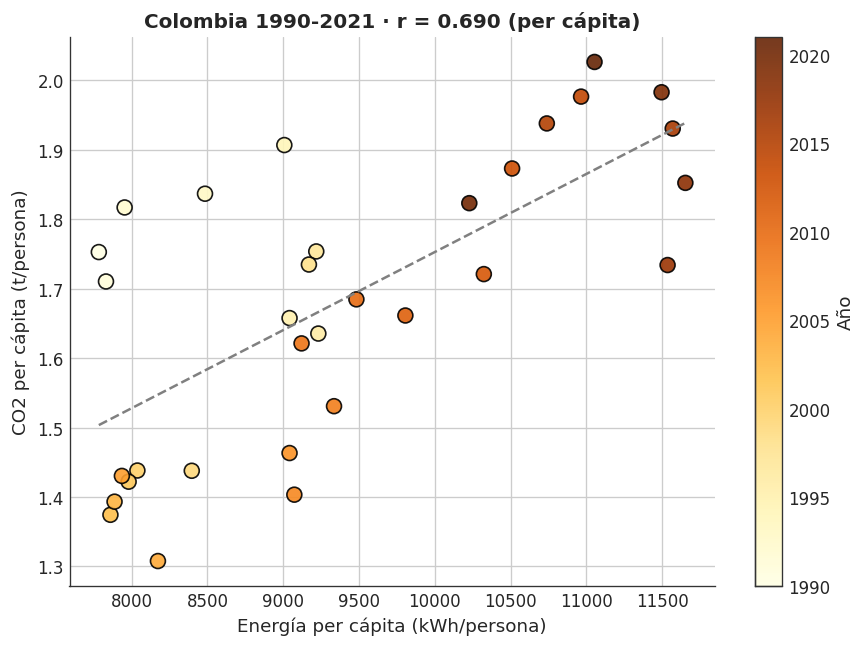
\includegraphics[width=0.48\textwidth]{figuras/scatter_energia_co2.png}
    \caption{Relación entre renovables (izq.) y energía per cápita (der.) con las emisiones de CO\textsubscript{2} per cápita.}
\end{figure}

\subsection*{Interpretación}
La energía consumida por habitante es, con diferencia, la variable más asociada a las emisiones totales (\textit{r} = 0.926), mientras que la participación renovable tiene una asociación negativa pero moderada con las emisiones per cápita. Esto sugiere que \textbf{el volumen de energía consumida pesa más que la composición de la matriz eléctrica} a la hora de explicar el crecimiento de las emisiones en Colombia.

% ===================== 7. HALLAZGOS Y PATRONES =====================
\section{Hallazgos de Patrones, Relaciones e Insights}

\begin{itemize}[leftmargin=1.2cm]
    \item El crecimiento de las emisiones de CO\textsubscript{2} en Colombia (+82\% entre 1990 y 2021) no está explicado principalmente por cambios en la matriz eléctrica renovable, que se mantuvo relativamente estable y siempre mayoritaria (61.8\%--83.9\%).
    \item El principal motor de las emisiones es el crecimiento del consumo de energía per cápita, asociado a la expansión económica, el transporte y la industria, sectores donde el país aún depende fuertemente de combustibles fósiles.
    \item La correlación negativa moderada entre renovables y CO\textsubscript{2} per cápita (\textit{r} = -0.601) indica que, si bien una mayor participación renovable sí se asocia con menores emisiones por habitante, su efecto es parcial: no compensa completamente el crecimiento del consumo energético total.
    \item Las caídas puntuales en la participación renovable (p. ej. 1992, 2015--2016) coinciden con periodos de menor disponibilidad hídrica, evidenciando la vulnerabilidad estructural de una matriz eléctrica dependiente en gran medida de la hidroelectricidad.
\end{itemize}

% ===================== 8. SELECCIÓN DEL MODELO =====================
\section{Selección del Modelo y Justificación de su Elección}

Dado que el conjunto de datos cuenta con un tamaño reducido ($n=32$ observaciones anuales) y solo dos variables predictoras (\texttt{Renewables\_pct} y \texttt{Energy\_per\_capita}), se optó por comparar seis modelos de regresión de distinta naturaleza, evaluados todos bajo el mismo esquema de validación:

\begin{itemize}[leftmargin=1.2cm]
    \item \textbf{Regresión Lineal, Ridge (L2) y Lasso (L1):} modelos lineales interpretables, útiles como referencia base y para cuantificar la dirección y magnitud del efecto de cada variable.
    \item \textbf{K-Nearest Neighbors (KNN):} modelo no paramétrico capaz de capturar relaciones no lineales entre las variables sin asumir una forma funcional específica.
    \item \textbf{Random Forest y Árbol de Decisión:} modelos basados en árboles, incluidos para explorar posibles relaciones no lineales adicionales, aunque con mayor riesgo de sobreajuste dado el tamaño muestral reducido.
\end{itemize}

\subsection*{Esquema de validación}
Debido al bajo número de observaciones, se utilizó validación cruzada \textbf{Leave-One-Out (LOOCV)}, que en cada iteración entrena el modelo con 31 años y predice el año restante, maximizando el uso de los datos disponibles y reduciendo el sesgo de una única partición entrenamiento/prueba.

\begin{figure}[h!]
    \centering
    \includegraphics[width=0.75\textwidth]{figuras/comparacion_modelos.png}
    \caption{Comparación de los 6 modelos evaluados mediante LOOCV.}
\end{figure}

\subsection*{Modelos seleccionados}
Con base en el desempeño (R\textsuperscript{2}, RMSE y MAE), se seleccionaron dos modelos para el análisis en detalle: \textbf{KNN (k=6)}, por ser el de mejor desempeño predictivo, y \textbf{Ridge (L2)}, por ofrecer coeficientes interpretables que permiten cuantificar la dirección del efecto de cada variable sobre las emisiones.

% ===================== 9. APLICACIÓN DEL MODELO =====================
\section{Aplicación del Modelo}

Ambos modelos se implementaron dentro de un \textit{pipeline} de \texttt{scikit-learn} que primero estandariza las variables predictoras (\texttt{StandardScaler}) y luego ajusta el modelo, evaluando siempre mediante LOOCV:

\begin{lstlisting}
X = df_clean[['Renewables_pct', 'Energy_per_capita']]
y = df_clean['CO2_per_capita']
loocv = LeaveOneOut()

modelo_ridge = Pipeline([('scaler', StandardScaler()),
                          ('model', Ridge(alpha=1.0))])

y_pred_ridge = cross_val_predict(modelo_ridge, X, y, cv=loocv)
r2_ridge = r2_score(y, y_pred_ridge)
\end{lstlisting}

Para KNN se realizó adicionalmente una búsqueda del hiperparámetro $k$ (número de vecinos) probando valores de 1 a 15 y seleccionando el que maximiza el R\textsuperscript{2} bajo LOOCV, resultando en $k=6$ como valor óptimo.

\begin{figure}[h!]
    \centering
    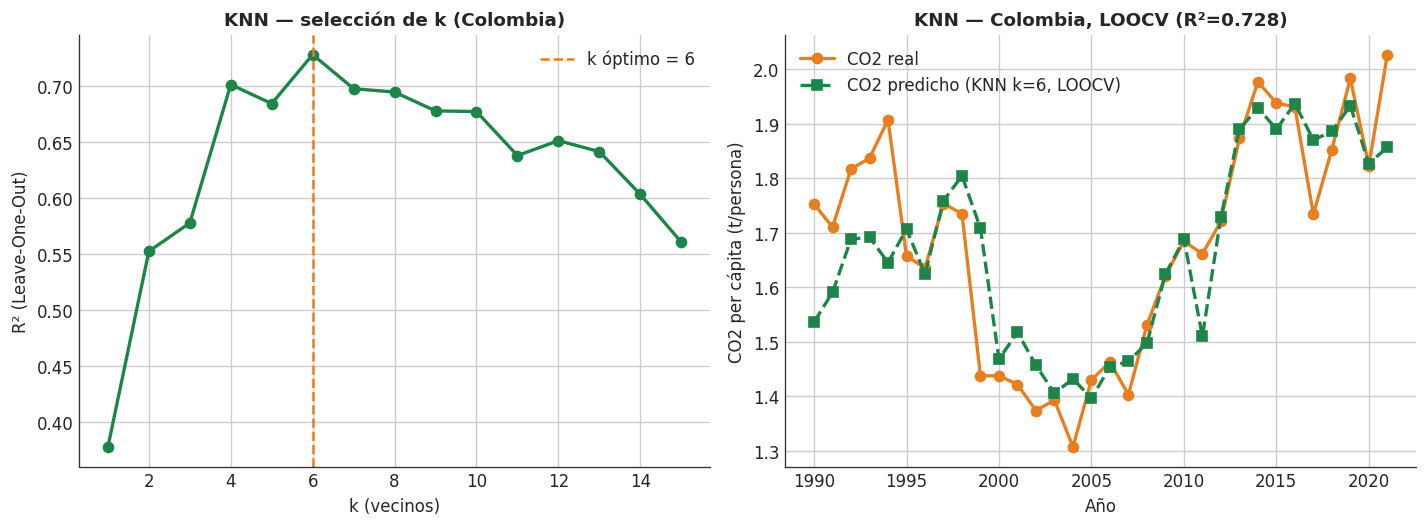
\includegraphics[width=\textwidth]{figuras/knn_resultados.png}
    \caption{Selección del hiperparámetro $k$ (izq.) y predicción vs. valor real bajo LOOCV (der.) para KNN.}
\end{figure}

% ===================== 10. EVALUACIÓN E INTERPRETACIÓN =====================
\section{Evaluación del Modelo e Interpretación de los Resultados}

\begin{center}
\begin{tabular}{@{}lccc@{}}
\toprule
\textbf{Modelo} & \textbf{R\textsuperscript{2}} & \textbf{RMSE} & \textbf{MAE} \\
\midrule
KNN (k=6)          & \textbf{0.728} & 0.107 & 0.076 \\
Ridge (L2)         & 0.692          & 0.114 & 0.093 \\
Regresión Lineal   & 0.692          & 0.114 & 0.093 \\
Lasso (L1)         & 0.688          & 0.115 & 0.094 \\
Random Forest      & 0.574          & 0.134 & 0.090 \\
Árbol de Decisión  & 0.419          & 0.156 & 0.114 \\
\bottomrule
\end{tabular}
\end{center}

El modelo \textbf{KNN (k=6)} obtuvo el mejor desempeño predictivo (R\textsuperscript{2}=0.728, el menor RMSE y MAE), superando a los modelos lineales. Los modelos de árboles (Random Forest y Árbol de Decisión) tuvieron el desempeño más bajo, consistente con su tendencia a sobreajustar en muestras pequeñas.

\begin{figure}[h!]
    \centering
    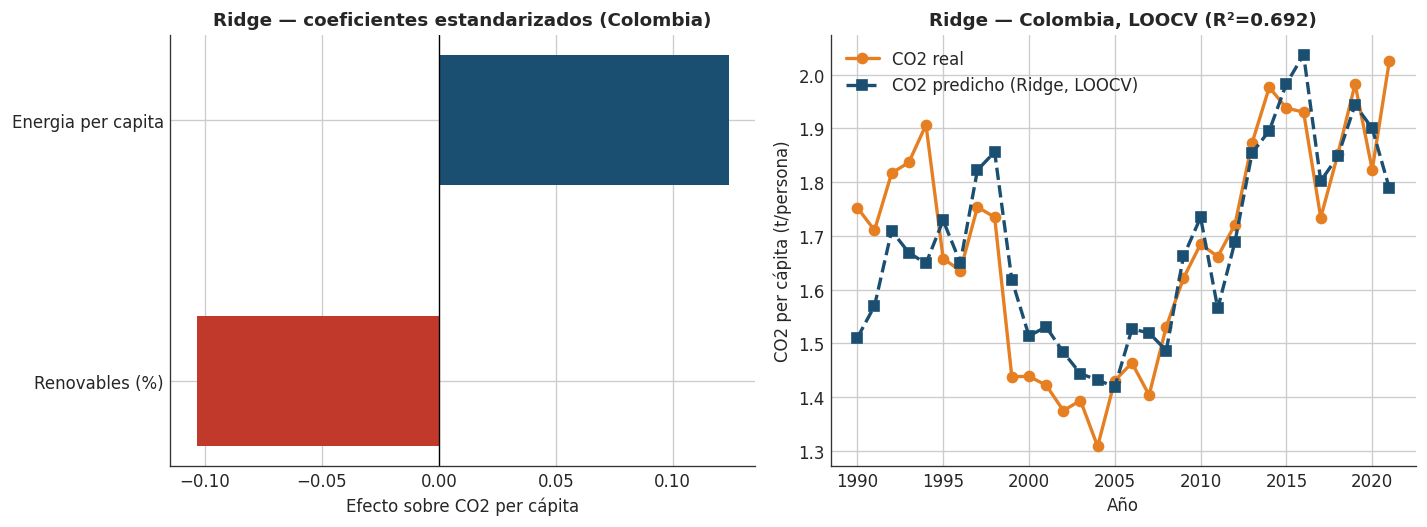
\includegraphics[width=\textwidth]{figuras/ridge_resultados.png}
    \caption{Coeficientes estandarizados del modelo Ridge (izq.) y predicción vs. valor real bajo LOOCV (der.).}
\end{figure}

Los coeficientes estandarizados del modelo Ridge confirman la dirección de las correlaciones encontradas en el análisis estadístico: el consumo de energía per cápita tiene un efecto \textbf{positivo} sobre las emisiones de CO\textsubscript{2} per cápita, mientras que la participación de renovables tiene un efecto \textbf{negativo}, de magnitud ligeramente menor.

\begin{figure}[h!]
    \centering
    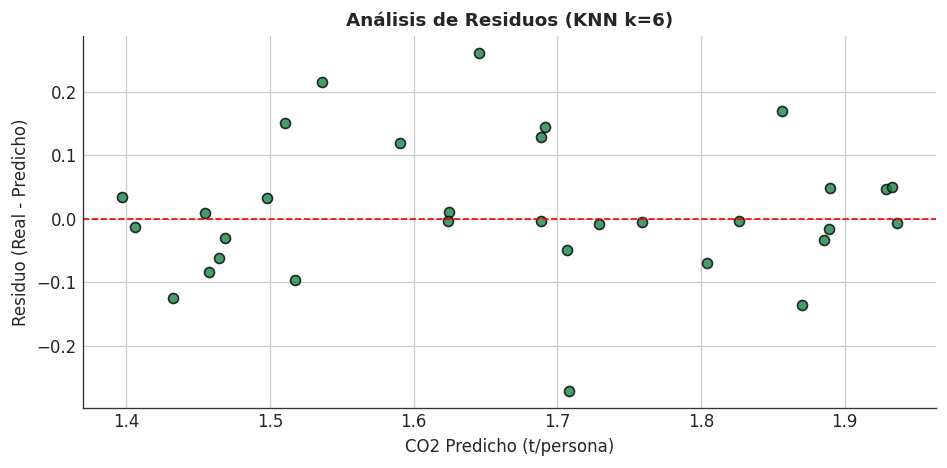
\includegraphics[width=0.75\textwidth]{figuras/residuos_knn.png}
    \caption{Análisis de residuos del modelo KNN (k=6).}
\end{figure}

El análisis de residuos del modelo KNN no muestra un patrón sistemático evidente (los residuos se distribuyen razonablemente alrededor de cero), aunque existen algunos años con mayor error de predicción, probablemente asociados a condiciones particulares (climáticas o económicas) no capturadas por las dos variables predictoras utilizadas.

% ===================== 11. CONCLUSIONES Y RECOMENDACIONES =====================
\section{Conclusiones y Recomendaciones}

\subsection*{Conclusiones}
\begin{itemize}[leftmargin=1.2cm]
    \item Existe una relación negativa moderada entre la participación de energías renovables y las emisiones de CO\textsubscript{2} per cápita en Colombia (\textit{r} = -0.601), pero esta relación por sí sola no explica el fuerte crecimiento de las emisiones totales observado entre 1990 y 2021.
    \item El principal factor asociado al crecimiento de las emisiones es el aumento del consumo de energía per cápita (\textit{r} = 0.690 con CO2 per cápita; \textit{r} = 0.926 con CO2 total), lo que indica que el problema es más de \textbf{volumen de consumo} que de \textbf{composición de la matriz eléctrica}.
    \item El modelo KNN (k=6) permitió predecir las emisiones de CO\textsubscript{2} per cápita con un ajuste razonable (R\textsuperscript{2}=0.728) a partir de únicamente dos variables energéticas, validando la relevancia de ambas variables para el fenómeno estudiado.
    \item La alta dependencia hidroeléctrica de Colombia genera vulnerabilidad frente a eventos climáticos (El Niño), que reducen momentáneamente la participación renovable y obligan a recurrir a generación térmica.
\end{itemize}

\subsection*{Recomendaciones}
\begin{itemize}[leftmargin=1.2cm]
    \item Diversificar la matriz renovable (solar y eólica) para reducir la dependencia hidroeléctrica y su vulnerabilidad climática.
    \item Enfocar la política de mitigación no solo en la generación eléctrica, sino en reducir la intensidad energética de sectores como transporte e industria, principales responsables del crecimiento del consumo total.
    \item Ampliar el análisis incorporando variables adicionales (PIB, emisiones por sector, participación de combustibles fósiles en transporte) que podrían mejorar la capacidad explicativa del modelo.
    \item Para trabajos futuros, aumentar el tamaño de la muestra (por ejemplo, mediante un panel de varios países de la región) permitiría construir modelos más robustos y generalizables que los obtenidos con $n=32$ observaciones de un solo país.
\end{itemize}

% ===================== 12. REFERENCIAS =====================
\section{Referencias}

\begin{enumerate}[leftmargin=1.2cm]
    \item[] Pedregosa, F., Varoquaux, G., Gramfort, A., Michel, V., Thirion, B., Grisel, O., Blondel, M., Prettenhofer, P., Weiss, R., Dubourg, V., Vanderplas, J., Passos, A., Cournapeau, D., Brucher, M., Perrot, M., \& Duchesnay, E. (2011). Scikit-learn: Machine learning in Python. \textit{Journal of Machine Learning Research, 12}, 2825--2830.
    \item[] Ritchie, H., Rosado, P., \& Roser, M. (2023). \textit{CO\textsubscript{2} and Greenhouse Gas Emissions} [Conjunto de datos]. Our World in Data. \url{https://github.com/owid/co2-data}
    \item[] Ritchie, H., Rosado, P., \& Roser, M. (2023). \textit{Energy} [Conjunto de datos]. Our World in Data. \url{https://github.com/owid/energy-data}
\end{enumerate}

\end{document}
